% =====================================================================
%  第 5 章 Floer 同调 §5.1–§5.2 —— ch05a（tr07）
%  页段：PDF 197–226（原书 p.187–216）
% =====================================================================
% [原文 p.187]
\chapter{Floer 同调}

\section{周期哈密顿系统与 Arnold 猜想}

\takeaway{本节把 1 周期解化为环路空间上泛函 $\mathcal{A}_h$ 的临界点（定理 5.5），并说明 $\mathcal{A}$ 的 Morse 指数为无穷大，故稳定与不稳定流形的老办法失效。Arnold 猜想断言 0 同伦的 1 周期解至少 $c(\oplus H_*(M;\Z))$ 个；Floer 的处方是把 $\mathcal{A}_h-\mathcal{A}$ 看作不含微分的紧项。}

Floer 基于 §2.5 所述的 Morse 理论与伪全纯曲线的关系，开创了“$\infty/2$ 维同调论”，即 Floer 同调（Floer homology），并给出了它在周期哈密顿系统以及拉格朗日子流形相交问题上的应用（[102]、[103]、[105]–[109]）。此后，Floer 本人（借助 Taubes [358] 的想法）又发现了基于 3 维流形规范理论的另一种 Floer 同调——3 维流形的 Floer 同调（[104]）。它与 4 维流形规范理论所给不变量的关系，由 Donaldson 等人阐明\footnote{关于规范理论中的 Floer 同调，参见 [126]。}。

Floer 同调是真正无穷维的不变量，在数学上被严格建立起来的“无穷维几何学”中是最深刻的理论，其可能性不可估量。本书概述周期哈密顿力学系统与拉格朗日子流形的 Floer 同调。

% [Tutor Note: “$\infty/2$ 维”是作者对 Morse 指数为无穷大这一现象的叫法：Floer 同调的次数只取 $\Z$ 或 $\Z_2$，但复形每个次数上有无穷多个生成元，介于偶数维（各次数有限）与奇数维（指数无穷）之间。全书反复用这一说法，参见 p.191 的注 5.8。]

首先叙述周期哈密顿系统与 §2.5 的 Morse 理论的关系。设 $(M,\omega_M)$ 为辛流形。§1.3、§2.2 中，对函数 $h\colon M\to\R$ 定义了
% [原文 p.188]
它生成的哈密顿向量场 $X_h$。再写一遍：在 Darboux 坐标下
\[
  X_h=\sum_i\left(\frac{\partial h}{\partial p_i}\frac{\partial}{\partial q_i}-\frac{\partial h}{\partial q_i}\frac{\partial}{\partial p_i}\right)
\]
下文考虑 $h$ 依赖时间 $t$、且关于 $t$ 为周期的情况。即 $h\colon M\times S^1\to\R$。置 $h_t(x)=h(x,t)$。$X_{h_t}$ 是随时间 $t\in S^1$ 变化的向量场。常微分方程
\begin{equation}
  \frac{d\ell}{dt}=X_{h_t} \tag{5.1}
\end{equation}
称为\textbf{周期哈密顿系统}（periodic Hamiltonian system）。(5.1) 的 1 周期解（1 periodic solution），即满足 (5.1) 的 $\ell\colon S^1\to M$，是本章的主要研究对象。

在此之前，先说完全辛同胚。设 $h\colon M\times[0,1]\to\R$ 为光滑函数（不假定 $h(x,0)=h(x,1)$）。以 $X_{h_t}$ 为哈密顿向量场。对任意点 $p$，常微分方程 (5.1) 满足初始条件 $\ell_p(0)=p$ 的解 $\ell_p$ 唯一存在。

\begin{definition}{5.1}
  辛同胚 $\phi$ 称为\textbf{完全辛同胚}（exact symplectic diffeomorphism），是指存在 $h\colon M\times[0,1]\to\R$ 使 $\phi(p)=\ell_p(1)$ 成立。
\end{definition}

下一个引理由定理 2.18 显然可得。

\begin{lemma}{5.2}
  若 $H_1(M;\R)=0$，则完全辛同胚全体与辛同胚全体所成群的连通分支一致。
\end{lemma}

与周期哈密顿系统的关系如下。

\begin{lemma}{5.3}
  对任意完全辛同胚 $\phi\colon M\to M$，存在周期哈密顿函数 $h\colon M\times S^1\to\R$，使 $\phi$ 的不动点 $\{x\in M\mid\phi(x)=x\}$ 与 $h$ 所生成哈密顿系统的 1 周期解一一对应。
\end{lemma}

证明容易，故省略。由引理 5.3，研究完全辛同胚的不动点集，与研究周期哈密顿系统的 1 周期解集等价。本书研究后者。

% [原文 p.189]
辛同胚何时是完全的，可用 Calabi 不变量（Calabi invariant [55]）等判定。关于 Calabi 不变量，[31]、[254] 等有详述。（§6.6 将提到的通量猜想与 Calabi 不变量关系密切。）

回到周期哈密顿系统的研究。我们的方法是变分法。把 §2.5 考虑的泛函 $\mathcal{A}$ 稍作变形。

\begin{definition}{5.4}
  $\mathcal{A}_h(\ell)=\mathcal{A}(\ell)+\int_{S^1}h(\ell(t))dt$。
\end{definition}

下一个定理由 Hamilton 本人给出，可上溯到辛几何本身的起源。

\begin{theorem*}{5.5}
  $\ell$ 是泛函 $\mathcal{A}_h$ 的临界点，与 $\ell$ 是 (5.1) 的周期解等价。
\end{theorem*}

\begin{proof}
  取 $V$ 为 $\ell^*TM$ 的截面，置 $\ell_\tau(t)=\exp_{\ell(t)}(\tau V(t))$。则
  \begin{align*}
    \left.\frac{\partial\mathcal{A}_h(\ell_\tau)}{\partial\tau}\right|_{\tau=0}
    &=\int_{S^1}\omega\Bigl(V,\frac{\partial\ell}{\partial t}\Bigr)dt+\int_{S^1}(Vh_t)(\ell)dt\\
    &=\int_{S^1}\omega\Bigl(V,\frac{\partial\ell}{\partial t}\Bigr)dt-\int_{S^1}\omega(V,X_{h_t})dt
  \end{align*}
  此式对任意 $V$ 都为 0，与 (5.1) 等价。
\end{proof}

要求 (5.1) 的 1 周期解，只须寻找泛函 $\mathcal{A}_h$ 的临界点。

泛函 $\mathcal{A}_h$ 是环路空间 $\Omega_0(M)$ 上的（多值）函数。§2.6 中讨论了从曲面出发的映射所成空间上的泛函，即能量的临界点——调和映射；那里也出现了有限维不会发生的现象，即气泡。泛函 $\mathcal{A}_h$ 其实比能量还要无限维得多。下面说明它在哪里如此。

为了能具体计算，取 $M=T^{2n}=\C^n/\Z^{2n}$，即环面。（辛结构 $\omega_{T^{2n}}$ 取由 $\C^n$ 上通常复结构所确定的那个。）$\ell\colon S^1\to T^{2n}$ 可作 Fourier 级数展开为
% [原文 p.190]
\begin{equation}
  \ell(t)=\sum_ka_k\exp(2\pi\sqrt{-1}kt) \tag{5.2}
\end{equation}
这里 $a_k\in\C^n$，但只有 $a_0$ 是 $a_0\in\C^n/\Z^{2n}$。换言之，(5.2) 给出“同构”
\begin{equation}
  \Omega_0(T^{2n})\simeq T^{2n}\times\prod_{k\in\Z-\{0\}}\C^n \tag{5.3}
\end{equation}
当然，实际上必须赋予拓扑来考虑，故这个“同构”并不太严格。用 (5.3) 的坐标计算泛函 $\mathcal{A}$，得：

\begin{lemma*}{5.6}
  对 (5.2) 的 $\ell$，$\mathcal{A}(\ell)=\sum 2\pi k|a_k|^2$。
\end{lemma*}

\begin{proof}
  置
  \[
    u(re^{2\pi\sqrt{-1}t})=a_0+\sum_{k\ne0}a_kr\exp(2\pi\sqrt{-1}kt),
  \]
  则 $u\colon D^2\to T^{2n}$ 在 $S^1$ 上与 $\ell$ 一致。容易看出
  \[
    \int_{D^2}u^*\omega_{T^{2n}}=\sum 2\pi k|a_k|^2.
  \]
\end{proof}

\begin{remark}{5.7}
  $u$ 的能量是 $\sum 2\pi^3k^2|a_k|^2$。与引理 5.6 相比，只差在系数大体上变成了平方，但这个差别极大。
\end{remark}

% [Tutor Note: 环面上的要点是 $k$ 取遍全体整数：$\mathcal{A}$ 的 Hessian 特征值为 $2\pi k$（重数 $2n$），$k<0$ 一侧有无穷多个负特征值，故 Morse 指数为无穷大。这正是有限维 Morse 理论失效、必须转向 Floer 同调的原因，也预示 (5.4) 中 $\operatorname{grad}\mathcal{A}$ 的积分曲线会有限时间发散。]

由引理 5.6，$\mathcal{A}$ 的临界点由 $a_k=0$（$k\ne0$）给出。即全体常值环路。进一步，$\mathcal{A}$ 是 Bott–Morse 函数，Hessian 的特征值为 $2\pi k$，各自的重复度为 $2n$。

值得注意的是，$k$ 取遍所有整数；特别地，负特征值重复度之和即 Morse 指数为无穷大。同时正特征值重复度之和也为无穷大。因此，必须研究的泛函是 Morse 指数为无穷大的 Bott–Morse 函数。

\begin{remark}{5.8}
  Morse 指数为无穷大的 Morse 理论出现于（从）奇数维流形（出发的映射空间）的情形。现在考察的是从 $S^1$ 出发的映射空间。
  % [原文 p.191]
  规范理论的情形也一样：4 维流形上的规范理论给出 Morse 指数有限的 Morse 函数，即 Yang–Mills 泛函，产生 Donaldson 不变量；与此相对，3 维流形上的规范理论则像 Chern–Simons 泛函（§4.3）那样，成为 Morse 指数无穷大的 Morse 理论，通向规范理论的 Floer 同调。
\end{remark}

% [Tutor Note: 注 5.8 把“维数为奇数”与“Morse 指数无穷大”对应起来，其判据是 Hessian 在无穷多个方向上的符号。作者的类比是：4 维规范理论（Yang–Mills）指数有限，故有 Donaldson 不变量；3 维规范理论（Chern–Simons）指数无穷，故只有 Floer 同调这种 $\infty/2$ 维理论。]

奇数维与偶数维的这一差异，已经出现在指数定理中。Atiyah–Singer 指数定理（关于作为数的指数的定理）在奇数维包含的信息不多。取而代之，在奇数维重要的是 eta 不变量（eta invariant）的理论（[22]），它提取的仍然是 $\infty/2$ 维的量（就 eta 不变量而言是线性理论）。

要把这套办法用到周期哈密顿系统上，必须研究的不是 $\mathcal{A}$ 而是 $\mathcal{A}_h$。即使在环面的情形，直接计算 $\mathcal{A}_h$ 也很麻烦。

然而值得注意的是，$\mathcal{A}_h-\mathcal{A}$ 是积分 $\int_{S^1}h(\ell(t))dt$。这种可写成积分的量，与含有 $\ell$ 的微分的 $\mathcal{A}$ 相比，要温和得多。

用线性情形的比喻来说，相当于 $\mathcal{A}$ 的是给出算子象征的主部（含微分的部分），$\mathcal{A}_h-\mathcal{A}$ 的部分则是不含微分的紧算子部分。指数理论中的重要事实是：像指数这样的拓扑的（连续形变下不变的）量，由主部即象征决定。

假定这个类比在非线性的我们的情形也成立。那么，若有从 $\mathcal{A}$ 提取某种“拓扑的”东西的处方，则用同一处方从 $\mathcal{A}_h$ 提取，也应当得到同样的东西。Floer 同调的想法如下。

\textbf{处方 5.9}
\begin{enumerate}[label=（\arabic*）,leftmargin=2.8em]
  \item 以泛函临界点的信息与另一个信息（后文说明）为基础，作同调群。
  \item 所得同调群对泛函加“紧扰动”不变。

  % [原文 p.192]
  \item 考虑泛函为 $\mathcal{A}$ 的情形，获得关于 (1) 的同调群的信息。
  \item 考虑泛函为 $\mathcal{A}_h$ 的情形，用 (3) 与 (2) 得到的同调群信息，获得关于 $\mathcal{A}_h$ 临界点的信息。
\end{enumerate}
\hfill$\square$

% [Tutor Note: 处方 5.9 是本节的方法论总纲，并非定理。其第 (2) 条中的“紧扰动”指形如 $\mathcal{A}_h-\mathcal{A}$ 的不含微分的项：正因如此，$\mathcal{A}$ 与 $\mathcal{A}_h$ 才能定义出同一个同调不变量，“从 $\mathcal{A}$ 算出、对 $\mathcal{A}_h$ 可用”这条路线才成立。]

这样得到的，就是与 Arnold 猜想（[9]、[10]）相关的诸结果。原本的 Arnold 猜想如下。

\begin{conjecture}{5.10}
  设 $c_M$ 为 $M$ 上遍取所有函数的临界点个数的下界。则 $M$ 上任意的周期哈密顿系统 (5.1) 至少有 $c_M$ 个 0 同伦的 1 周期解。
\end{conjecture}

当哈密顿函数 $h$ 不依赖 $t$ 时，对 $h$ 的临界点 $p$，存在周期解 $\ell(t)\equiv p$。因此猜想 5.10 在此情形是显然的。

用 Morse 理论可以得到关于数 $c_M$ 的各种信息。典型的是 Morse 不等式：当 $h$ 是 Morse 函数时，$h$ 的临界点个数不小于 $M$ 的 Betti 数之和。若同调群有挠（torsion），则可得到比 Betti 数估计更精细的结论（推论 5.19）。

下面把泛函是 Morse 函数这一性质，翻译到周期哈密顿系统的情形。设 $h\colon M\times S^1\to\R$ 为哈密顿函数。把它看作 $h\colon M\times[0,1]\to\R$，取定义 5.1 确定的 $\phi$。$\phi$ 的不动点对应于 $h$ 所确定周期哈密顿系统的 1 周期解。$\phi$ 的不动点对应于 $\phi$ 的图像 $\operatorname{Graph}(\phi)$ 与对角线集 $M=\Delta_M\subset M\times M$ 的交点。

\begin{definition}{5.11}
  1 周期解称为\textbf{非退化}（nondegenerate），是指对应的交点 $\in\Delta_M\cap\operatorname{Graph}(\phi)$ 处 $\Delta_M$ 与 $\operatorname{Graph}(\phi)$ 横截相交。
\end{definition}

给定分次\footnote{这里考虑的是 $\Z_2$ 上的次数。也就是说，$H_*$ 分为两块，如 $H_*=H_0\oplus H_1$。}交换群 $H_*$ 时，如下定义 $c(H)$。考虑分次自由 $\Z$ 模 $C_*$ 与 $\partial\colon C_*\to C_{*-1}$，使 $\Ker\partial/\Image\partial\cong H_*$。$c(H)$ 是遍取这样的 $(C,\partial)$ 所得的 $\rank C$ 的最小值。

% [原文 p.193]
\begin{conjecture}{5.12}
  对 $M$ 上所有 0 同伦的 1 周期解都非退化的周期哈密顿系统，0 同伦的 1 周期解的个数不小于 $c(\oplus H_*(M;\Z))$。
\end{conjecture}

存在退化 1 周期解时对 1 周期解个数的估计，是估计一般（未必是 Morse 函数）函数的临界点个数这一问题在环路空间上的类比。

Lyusternik–Snirel'man 的范畴（category）理论，用杯积长度（cup length）等估计临界点个数\footnote{[239]。日文解说见 [368]。}。更高阶的杯积（Massey 积（Massey product）等）与上同调运算（cohomology operation [349]\footnote{日文解说见 [282]。}）也同样可用于估计。

这些还没有怎么用到基本群的非交换性；但也有积极利用基本群非交换性的估计（[96]）。

由于必须把这些诸问题都纳入视野，猜想 5.10 离解决还很远，但部分解很多。下面叙述其中几个。

最初的重要突破口\footnote{对 Weinstein 猜想的 Rabinowitz 与 Weinstein 的结果在先。}是 Conley–Zehnder [61]，把它与后来 Chapteron [59] 的结果合起来，就完全解决了 $T^{2n}$ 情形下的猜想 5.10、5.12。（$C_{T^{2n}}=2n+1$，$c(\oplus H_*(T^{2n};\Z))=2^{2n}$。）其次解决的是 $\CP^n$ 与黎曼面的情形。（由 Floer [101]、Sikorav [334] 等。$C_{\CP^n}=c(\oplus H_*(\CP^n;\Z))=n+1$。）

然后，大的进展是 Floer 发现的 Floer 同调。Floer 本人应用它，在单调辛流形的情形证明了猜想 5.12。Floer 的方法经 Hofer–Salamon [183] 与 Ono [293] 改进，在半正辛流形的情形解决了猜想 5.10（定理 5.14）。此后，Fukaya–Ono [124]、Liu–Tian [237]、Ruan [317] 对一般辛流形的情形，给出了比猜想 5.10 弱的、用有理数域上 Betti 数的估计（定理 5.15）。

% [原文 p.194]
下面就上面用到的术语作说明，并准确叙述定理。以下只考虑紧辛流形。对 $\beta\in\pi_2(M)$，用下式定义 Chern 数 $c^1(\beta)$ 与能量 $\mathcal{E}(\beta)$。
\[
  c^1(\beta)=\int_{S^2}\beta^*c^1(M),\qquad
  \mathcal{E}(\beta)=\int_{S^2}\beta^*\omega_M.
\]

\begin{definition}{5.13}
  $2n$ 维辛流形 $M$ 称为\textbf{单调}（monotone），是指存在正数 $\lambda$ 使 $c^1(\beta)=\lambda\mathcal{E}(\beta)$。

  $M$ 称为\textbf{半正}（semipositive），是指不存在 $\beta\in\pi_2(M)$ 满足 $\mathcal{A}(\beta)>0$ 且 $0>c^1(\beta)\ge6-2n$。
\end{definition}

% [Tutor Note: 定义 5.13 的第二句把能量写成 $\mathcal{A}(\beta)$，而本页上文正把能量记作 $\mathcal{E}(\beta)$；作者在 p.203 也以 $\mathcal{A}$ 称能量。读时按 $\mathcal{E}(\beta)>0$ 理解即可，译文照录原书。半正条件的实质是：能量为正的球面类中不存在 $c^1$ 取小负值者。]

单调则半正。

\begin{theorem}{5.14}
  设 $M$ 半正。则对 $M$ 上所有 0 同伦的 1 周期解都非退化的周期哈密顿系统，0 同伦的 1 周期解的个数不小于 $c(\oplus H_*(M;\Z))$。
\end{theorem}

\begin{theorem}{5.15}
  对任意辛流形上所有 0 同伦的 1 周期解都非退化的周期哈密顿系统，0 同伦的 1 周期解的个数不小于 $\sum_k\rank H_k(M;\Q)$\footnote{最近（1999 年 6 月），笔者与小野薰氏在定理 5.15 的假定下定义了整数系数的 Floer 同调，把定理 5.15 的结论强化到与定理 5.14 相同。详细结果将于近期发表，本书不予叙述，故本书把定理 5.15 写成有理数系数。}。
\end{theorem}

允许退化周期解时的讨论更为微妙。本书不涉及。

\section{Floer 同调}

\takeaway{本节把 Morse 理论升级为 Floer 同调：不追踪稳定与不稳定流形，只用连接两临界点的梯度流模空间 $\mathcal{M}(p,q;f)$ 定义边界算子 $\delta$；无穷维情形改用方程 (5.8)。困难在于虚拟维数随分支变化与紧致性缺失，对策是 Novikov 环与能量有界的截断 $\mathcal{M}(R_i,R_j;h;E)$。}

回到前面所述的处方 5.9，解说定理 5.14、5.15 证明的主要想法。

从 Morse 函数恢复流形同调的方法，已经出现在第 3 章定理 3.17 的证明中。第 3 章用了稳定流形与不稳定流形。对 $\mathcal{A}$ 而言，它们的存在是微妙的问题。最大的困难是 $\operatorname{grad}\mathcal{A}$、$\operatorname{grad}\mathcal{A}_h$ 生成的 1 参数变换群不存在。实际上，
% [原文 p.195]
设以 $\ell_0(t)=\sum_ka_k\exp(2\pi\sqrt{-1}kt)$ 为初值的积分曲线为
\begin{equation}
  \tau\mapsto\ell_\tau(t)=\sum_{k>0}a_k\exp(k\tau+2\pi\sqrt{-1}kt) \tag{5.4}
\end{equation}
则 (5.4) 只要 $a_k$ 除有限个之外不全为 0，就在有限时间内发散（由单复变函数论的 Liouville 定理可知）。而且，发散因 $a_k$ 的取法可以在任意接近 0 的地方发生，无法控制。

如此可知，用稳定流形等办法从 Morse 函数造同调论，对 $\mathcal{A}$ 极其困难。这源于前面所述 $\mathcal{A}$ 的特点，即 Morse 指数为无穷大。大概看到这一事实后，认为 $\mathcal{A}$ 不适合作展开 Morse 理论所用泛函的人，在 Floer 登场之前很多吧。

解决这一点的下述两个想法，原本以萌芽形式见于 Conley–Zehnder [61]，由 Floer 实现。

\textbf{想法 5.16}\quad 从 Morse 函数恢复同调，并不需要知道稳定流形与不稳定流形，即从一点出发（进入一点）的全部轨道。对两个临界点，只要知道连接它们的全部轨道即可。\hfill$\square$

\textbf{想法 5.17}\quad 对泛函 $\mathcal{A}_h$ 的两个临界点，若考虑连接它们且属于某个确定同伦类的全部轨道，其虚拟维数有限。\hfill$\square$

由这两个观察，实现处方 5.9(1)、从 $\mathcal{A}_h$ 的临界点作同调论的道路就打开了。下面更准确地叙述。

先说明 Morse–Witten 复形这一概念。回想定理 3.17。为了与哈密顿函数 $h$ 区别，Morse 函数记作 $f$。又，目的是考虑 $\Omega(M)$ 上的函数 $\mathcal{A}_h$，故 $f$ 所定义在的流形记作 $X$（而非 $M$）。

定理 3.17 考虑的是 Bott–Morse 函数，现在试把定理 3.17 用于 Morse 函数的情形。以下用上同调而不用同调。也就是说，把余维数 $k$ 的链看作 $k$ 次上链。曾为
\[
  E_2^k=\bigoplus_iH^k(N_i^{+},N_i^{+}-R_i;\Z).
\]
当 $f$ 是 Morse 函数时，$R_i$ 是一点 $p_i$，且 $N_i^{+}\simeq$
% [原文 p.196]
$\R^{n-\mu(p_i)}$（$\mu(p_i)$ 是 Morse 指数）。因此，$E_2^k$ 是以 Morse 指数为 $n-k$ 的临界点为生成元的自由交换群。记 $E_2^k=CF^k(X,f)$。即
\begin{equation}
  CF^k(X,f)=\bigoplus_{p\in\operatorname{Cr}(h),\ \mu(p)=n-k}\Z[p] \tag{5.5}
\end{equation}
$E_2^k$ 的元素经若干次微分相消后到达 $E_\infty^k$。考虑次数可知，这些微分汇总为 $CF^*(X,h)$ 上的边界算子
\[
  \delta\colon CF^k(X,f)\to CF^{k+1}(X,f)
\]
（此事后文用别的方法准确证明，故这里作稍粗的说明。）结果下述定理就得到了。

% [Tutor Note: 式 (5.5) 的下标作 $\operatorname{Cr}(h)$，两行后又作 $CF^*(X,h)$，而同页定理 5.18、系 5.19 与定义 5.25 都用 $f$（定义 5.25 的求和式中又混入 $\mathcal{M}(p,q;h)$）。按上下文，这几处的 $h$ 都应读作 Morse 函数 $f$：全书 $h$ 专指哈密顿函数。译文照录原书。]

\begin{theorem}{5.18}
  存在上链复形（cochain complex）$(CF^*(X,f),\delta)$，具有下述性质。
  \begin{enumerate}[label=（\arabic*）,leftmargin=2.8em]
    \item $\rank CF^k(X,f)$ 等于 $f$ 的 Morse 指数为 $n-k$ 的临界点个数。
    \item $(CF^*(X,f),\delta)$ 的上同调与 $X$ 的上同调一致。
  \end{enumerate}
\end{theorem}

\begin{corollary}{5.19}
  $M$ 上任一 Morse 函数的临界点个数不小于 $c(H_*(M;\Z))$。
\end{corollary}

现在想对 $f=\mathcal{A}_h$ 的情形构造定理 5.18 的复形。分次\footnote{这里次数取 $\Z$ 次数。}交换群 $CF^k(\Omega M,\mathcal{A}_h)$（Morse 指数的定义仍有问题）可以照样定义。问题在边界算子。有限维情形下它是连接同态
\[
  \delta\colon H_{\mu(p_i)}(\mathfrak{X}_i,\mathfrak{X}_{i-1};\Z)\to H_{\mu(p_i)-1}(\mathfrak{X}_{i-1};\Z)
\]
（见定理 3.17 的证明）。如前所述，把相当于 $\mathfrak{X}_i$ 的东西在我们的无穷维情形下定义出来是不可能的。因此，需要一种与连接同态不同的 $\delta$ 的描述。用连接两个临界点的梯度向量场积分曲线的模空间可以描述——这就是想法 5.17。

为了以后也能用于 Floer 同调的计算，下面在定义 5.20、引理 5.22 中也把 Bott–Morse 函数的情形包含进来。
% [原文 p.197]
设 $f$ 为 Bott–Morse 函数。确定黎曼度量，把 $f$ 的梯度向量场记作 $\operatorname{grad}f$。设 $R_i,R_j$ 是 $f$ 的临界点集的连通分量。

\begin{definition}{5.20}
  \[
    \tilde{\mathcal{M}}(R_i,R_j;f)=\left\{\gamma\colon\R\to X\ \middle|\
    \frac{d\gamma}{dt}=\operatorname{grad}f,\
    \lim_{\tau\to+\infty}\gamma(\tau)\in R_j,\
    \lim_{\tau\to-\infty}\gamma(\tau)\in R_i\right\}
  \]
  这里 $\lim_{\tau\to+\infty}\gamma(\tau)\in R_j$ 是指极限 $\lim_{\tau\to+\infty}\gamma(\tau)$ 存在且属于 $R_j$。
\end{definition}

以后为简单起见，把 $\lim_{\tau\to+\infty}\gamma(\tau)\in R_j$ 写作 $\gamma(\infty)\in R_j$。

\begin{remark}{5.21}
  以后为避免混乱，$\Omega_M$（或 $X$）中的道路及其参数用 $\gamma,\tau$，$M$ 中的道路及其参数用 $\ell,t$。
\end{remark}

若 $\operatorname{grad}f$ 生成的 1 参数变换群 $\varphi_\tau$ 存在，则用引理 3.22 之前引入的记号 $\varphi_\infty(x)$，有
\begin{equation}
  \tilde{\mathcal{M}}(R_i,R_j;f)=\{x\in X\mid\varphi_{-\infty}(x)\in R_i,\ \varphi_\infty(x)\in R_j\} \tag{5.6}
\end{equation}
然而，当 $f=\mathcal{A}_h$ 时，如前所述 $\varphi_\tau$ 没有定义，故应尽量避免 (5.6) 那样的写法，而用积分曲线 $\gamma$ 的语言记述。

% [Tutor Note: 作者刻意避开 (5.6)，是因为 $\operatorname{grad}\mathcal{A}_h$ 的流在 $L^2$ 意义下不可积：由 (5.4)，$\mathcal{A}$ 的流会有限时间发散，环路空间上根本没有整体定义的 $\varphi_\tau$。Floer 的做法是只在模空间层面用“连接轨道”定义 $\delta$，把流的整体存在性绕过去。]

$\tilde{\mathcal{M}}(R_i,R_j;f)$ 上有群 $\R$ 以 $(s\cdot\gamma)(\tau)=\gamma(s+\tau)$ 作用。若 $i\ne j$，作用自由。商空间记作 $\mathcal{M}(R_i,R_j;f)$。

暂时讨论有限维情形。以下一段引理的证明在 $f=\mathcal{A}_h$ 时不能用，但引理的结论本身在 $f=\mathcal{A}_h$ 时施以适当修正后成立。

\begin{lemma*}{5.22}
  把 Bott–Morse 函数 $f$ 在 $\operatorname{Cr}(f)$ 之外小幅移动，可使下述性质得到满足：$\tilde{\mathcal{M}}(R_i,R_j;f)$ 是流形，其维数为 $\dim R_j+\mu(R_j)-\mu(R_i)$。
\end{lemma*}

\begin{proof}
  $\gamma\mapsto\gamma(0)$ 给出 $\tilde{\mathcal{M}}(R_i,R_j;f)$ 与 $U(R_i)\cap S(R_j)$ 的同胚。可移动 $f$ 使 $U(R_i)$ 与 $S(R_j)$ 横截相交。于是
  % [原文 p.198]
  $\tilde{\mathcal{M}}(R_i,R_j;f)=U(R_i)\cap S(R_j)$ 是流形，维数为 $\dim U(R_i)+\dim S(R_j)-n$。因 $\dim U(R_i)=n-\mu(R_i)$、$\dim S(R_j)=\dim R_j+\mu(R_j)$，引理成立。
\end{proof}

以下取 $f$ 满足引理 5.22 的条件。为简单起见，设 $R_i$ 与向量丛 $N_i^{-}\to R_i$ 可定向\footnote{也可以去掉这个条件，但那样定向的讨论会更微妙。此外，笔者的论文 [117] 在这一点上有错误。}。

\begin{lemma*}{5.23}
  $\tilde{\mathcal{M}}(R_i,R_j;f)$ 上有定向。定向由 $R_i$、$R_j$ 的稳定流形的定向决定。
\end{lemma*}

\begin{proof}
  为简单起见设 $X$ 可定向。则由 $X$ 的定向与 $U(R_i)$ 的定向，$S(R_i)$ 上得到定向。故由 $\tilde{\mathcal{M}}(R_i,R_j;f)\simeq U(R_i)\cap S(R_j)$ 引理成立。（即使 $X$ 没有定向，引理 5.23 也成立。参见 [124] Remark 22.5。）
\end{proof}

完成边界算子的描述。设 $f$ 为 Morse 函数。取 $p,q\in\operatorname{Cr}(h)$，$\mu(p)=\mu(q)+1$。由引理 5.22、5.23，$\tilde{\mathcal{M}}(p,q;f)$ 是 1 维定向流形。因 $\R$ 自由作用，连通分量与 $\R$ 同胚。这里需要下述引理。

\begin{lemma}{5.24}
  若 $\mu(p)+1=\mu(q)$，则 $\mathcal{M}(p,q;f)$ 紧。
\end{lemma}

证明稍后叙述。$\mathcal{M}(p,q;f)$ 的元素 $[\gamma]$ 对应于 $\tilde{\mathcal{M}}(p,q;f)$ 的连通分量。当对应连通分量的定向与 $\R$ 的作用相容时置 $\epsilon(\gamma)=+1$，否则置 $\epsilon(\gamma)=-1$。

\begin{definition}{5.25}
  \[
    \langle\delta p,q\rangle=\sum_{[\gamma]\in\mathcal{M}(p,q;h)}\epsilon(\gamma),
  \]
  \[
    \delta[p]=\sum_{q\in\operatorname{Cr}(f),\ \mu(q)=\mu(p)+1}\langle\delta p,q\rangle[q].
  \]
  称 $(CF(M,f),\delta)$ 为\textbf{Morse–Witten 复形}（Morse-Witten complex）。
\end{definition}

\begin{theorem}{5.26}
  $\delta\delta=0$，且 $(CF(X,f),\delta)$ 的上同调与 $X$ 的上同调一致。
\end{theorem}

% [原文 p.199]
\begin{remark}{5.27}
  定义 5.25 的构造很古老，可上溯到 Morse 本人。Thom [362] 也是重要贡献，Smale 对高维 Poincaré 猜想的证明也与定理 5.26 密切相关。又，Milnor 的名著教科书 [258] 的记述与定理 5.26 非常接近。Witten 在 [391] 中叙述了接近定理 5.26 的构造，并阐明了它与超对称场论的关系\footnote{参见 [135]。}。看透用 $\mathcal{M}(p,q;f)$ 不用稳定流形等也能表出同调的人，大概是 Conley–Zehnder。把定理 5.26 形式的定理本身（包括整数系数情形）明确叙述出来的，是 Floer。（Witten 考虑的是实数系数。）
\end{remark}

叙述定理 5.26 证明的梗概。先证 $\delta\delta=0$。为此用 $\mu(p)+2=\mu(q)$ 情形的模空间 $\mathcal{M}(p,q;f)$。$\mathcal{M}(p,q;f)$ 是定向的 1 维流形。

\begin{lemma}{5.28}
  设 $\mu(p)+2=\mu(q)$。则存在 $\mathcal{M}(p,q;f)$ 的紧化 $\mathcal{CM}(p,q;f)$，并存在定向 0 维流形之间的同胚
  \[
    \partial\mathcal{CM}(p,q;f)=\bigcup_{r\in\operatorname{Cr}(f),\ \mu(p)+1=\mu(r)}\mathcal{M}(p,r;f)\times\mathcal{M}(r,q;f).
  \]
\end{lemma}

承认引理 5.28，则作为 1 维流形边界的 0 维流形的“带号的位数”为 0，故
\[
  \sum_{r\in\operatorname{Cr}(f),\ \mu(p)+1=\mu(r)}\langle\delta p,r\rangle\langle\delta r,q\rangle=0
\]
成立。因此 $\delta\delta=0$。

其次叙述引理 5.24、5.28 证明的梗概。设 $\gamma_i\in\tilde{\mathcal{M}}(p,q;f)$，$[\gamma_i]$ 在 $\mathcal{M}(p,q;f)$ 中发散。

设 $f(p)<s<f(q)$。因 $\tau\mapsto f(\gamma_i(\tau))$ 单调增加，存在唯一的 $m_i(s)\in\R$ 使 $f(\gamma_i(m_i(s)))=s$ 成立。

$\operatorname{Cr}(f)$ 是有限集。把 $\{f(r)\mid r\in\operatorname{Cr}(f)\}$ 与闭区间 $[f(p),f(q)]$ 的交记作 $\{r_1,\dots,r_J\}$，$r_1<r_2<\cdots<r_J$。则 $r_1=f(p)$，$r_J=f(q)$。

% [原文 p.200]
\[
  1=\frac{dm_i}{ds}\frac{df\circ\gamma_i}{d\tau}(m_i(s))
\]
故若 $s\notin\{r_1,\dots,r_J\}$，则 $\dfrac{dm_i}{ds}(s)$ 不依赖 $i$ 而一致有界。于是可换子列，使存在 $\tau_{ij}\in\R$，$s\mapsto m_i(s)+\tau_{ij}$ 在区间 $(r_j,r_{j+1})$ 上广义一致收敛。

当 $\dfrac{dm_i}{ds}(r_j)$（$1<j<J$）发散时，取子列则 $\gamma_i(m_i(r_j))$ 收敛到 $\operatorname{Cr}(f)$ 的点。

当 $\dfrac{dm_i}{ds}(r_j)$ 收敛时，$s\mapsto m_i(s)+\tau_{ij}$ 在 $r_j$ 也收敛。于是把区间 $(r_{j-1},r_j)$ 与 $(r_j,r_{j+1})$ 连接成 $(r_{j-1},r_{j+1})$。

结果，存在有限个 $r'_j$（$j=1,\dots,J'$）与列 $\tau'_{ij}$，使 $\gamma_i(m_i(r'_j))$ 收敛到 $\operatorname{Cr}(f)$ 的点 $x_j$，且 $s\mapsto m_i(s)+\tau'_{ij}$ 在区间 $(r'_j,r'_{j+1})$ 上广义一致收敛（图 5.1）。于是取子列，$t\mapsto\gamma_i(\tau+\tau'_{ij})$ 收敛到 $\tilde{\mathcal{M}}(x_j,x_{j+1};f)$ 的元素。特别地，$\mathcal{M}(x_j,x_{j+1};f)$ 非空。故由引理 5.22，下述不等式成立。
\begin{equation}
  \mu(x_j)<\mu(x_{j+1}) \tag{5.7}
\end{equation}

现在设 $\mu(p)+1=\mu(q)$。由 (5.7) 与 $x_1=p$、$x_{J'}=q$，必须 $J'=2$。这与 $[\gamma_i]$ 是发散列矛盾。即 $\mathcal{M}(p,q;f)$ 紧。这就证明了引理 5.24。

其次设 $\mu(p)+2=\mu(q)$。则 $J'=3$，作为列 $[\gamma_i]$ 的极限，得到 $\mathcal{M}(p,x_2;f)$ 的元素与 $\mathcal{M}(x_2,q;f)$ 的元素之组。也就是说，把引理 5.28 的右边添上，$\mathcal{M}(p,q;f)$ 就被紧化。

\begin{remark}{5.29}
  以上证明中用 Morse 函数的值重取参数的技巧，是古田幹雄氏教给我的。
\end{remark}

为证明引理 5.28，尚须说明的是：$\mathcal{M}(p,r;f)\times\mathcal{M}(r,q;f)$ 的任意点“附近”存在与 $(T,\infty)$ 同胚的 $\mathcal{M}(p,q;f)$ 的一部分（$T$ 是大的正数），以及定向。前者的证明，即使在有限维 Morse 理论的情形，也需要做 Taubes 在 [357] 中对规范理论情形所做的同样的粘接论证\footnote{关于此点 [328] 中有证明，但只为有限维情形去详细学习这个证明，所得恐怕与所费功夫不相称。另一方面，[176] 对定理 5.26 有出色的解说，但省略了这一点的说明。}。

% [原文 p.201]
\begin{figure}[htbp]
  \centering
  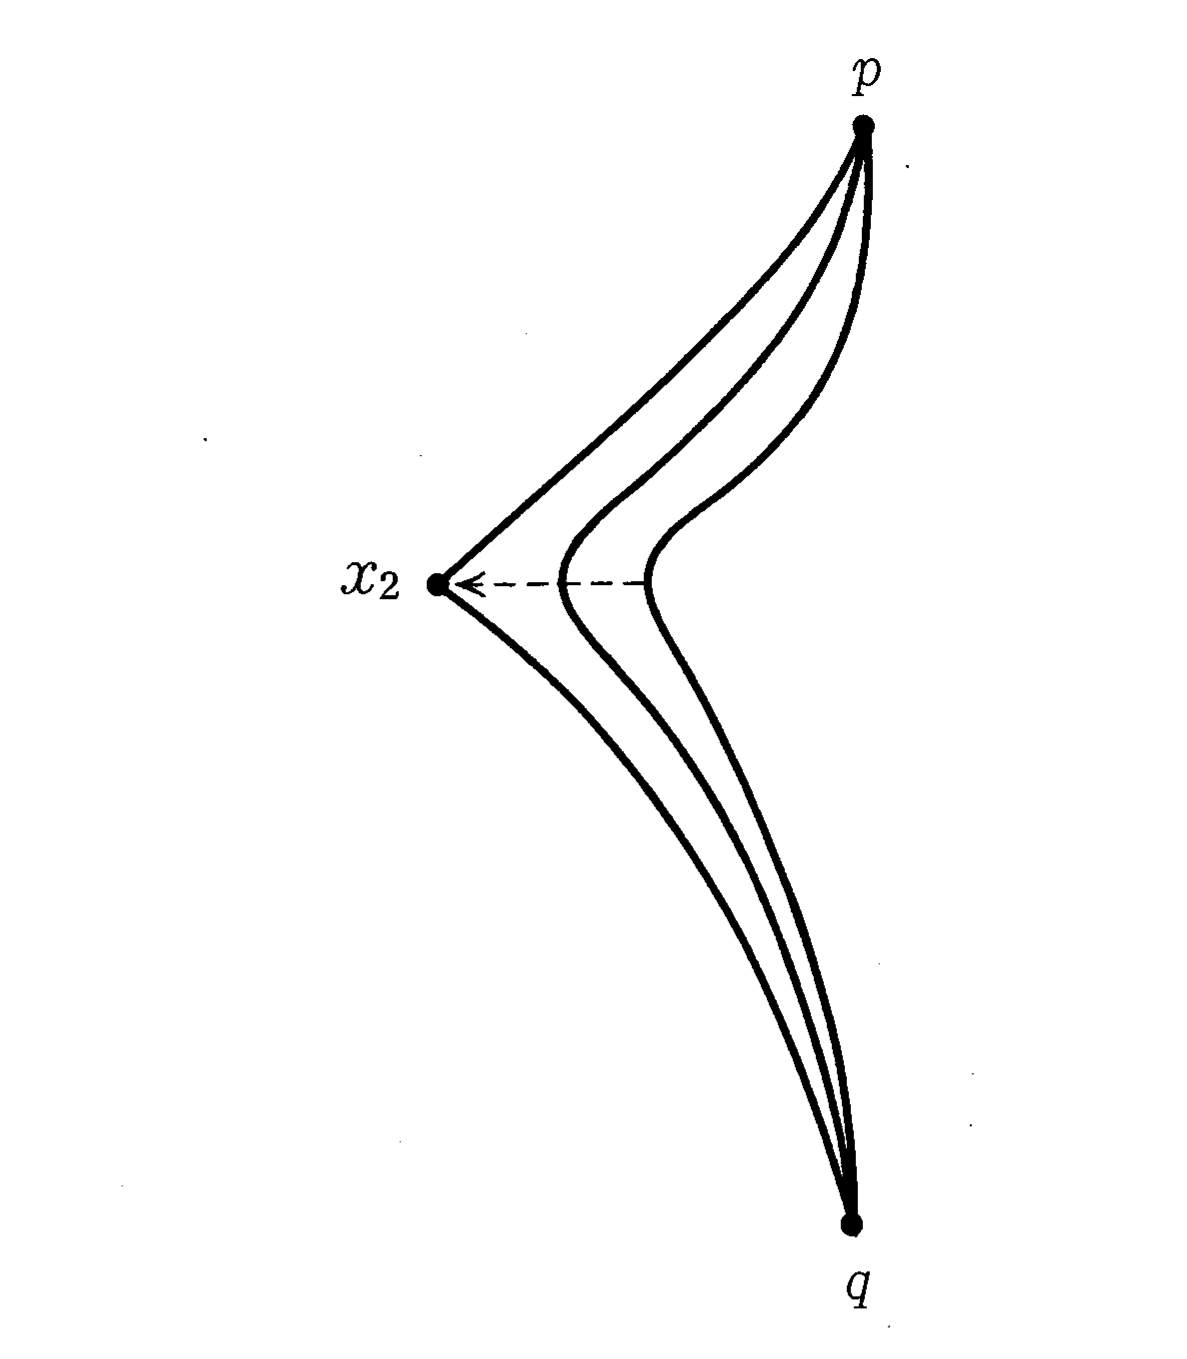
\includegraphics[width=0.55\textwidth]{figures/fig5.1.png}
  \figtitle{5.1}{$\mathcal{M}(p,q;f)$ 的紧化（原书 p.201）}
\end{figure}

这部分省略。

为完成定理 5.26 的证明，必须证明 $(CF(M,f),\delta)$ 的上同调与 $M$ 的上同调一致。这一点留待 §5.3 说明，先把话题移到无穷维情形（$f=\mathcal{A}_h$ 的情形）。

首先改写 $\gamma\colon\R\to\Omega_0(M)$ 是 $\operatorname{grad}\mathcal{A}_h$ 的积分曲线这一条件。设 $\gamma(\tau)=\ell_\tau\colon S^1\to M$。置 $\tilde\gamma(\tau,t)=\ell_\tau(t)$。则 $\tilde\gamma\colon\R\times S^1\to M$。

\begin{lemma*}{5.30}
  $\gamma$ 是 $\operatorname{grad}\mathcal{A}_h$ 的积分曲线，与下式等价。
  \begin{equation}
    \frac{\partial\tilde\gamma}{\partial\tau}
    +J_M\left(\frac{\partial\tilde\gamma}{\partial t}-X_{h_t}\right)=0. \tag{5.8}
  \end{equation}
\end{lemma*}

\begin{proof}
  用定理 5.5 证明中的记号，则
  \begin{align*}
    \left.\frac{\partial\mathcal{A}_h(\ell)}{\partial\tau}\right|_{\tau=0}
    &=-\int_{S^1}\omega\Bigl(\frac{\partial\ell}{\partial t},V\Bigr)dt
      -\int_{S^1}\omega(X_{h_t},V)dt\\
    &=-\int_{S^1}g_M\Bigl(J_M\Bigl(\frac{\partial\tilde\gamma}{\partial t}-X_{h_t}\Bigr),V\Bigr)dt
  \end{align*}

  % [原文 p.202]
  由 $\tilde g_M(V,W)=\int_{S^1}g_M(V,W)dt$ 是 $\Omega_0M$ 的黎曼度量，引理成立。
\end{proof}

% [Tutor Note: (5.8) 的推导要点是：在 $L^2$ 内积 $\tilde g_M$ 下，$\operatorname{grad}\mathcal{A}_h$ 的那一项正好是 $J_M(\partial_t\tilde\gamma-X_{h_t})$；$h=0$ 时它就是 $\bar\partial$ 方程。这正是 §2.5 把伪全纯曲线看成环路空间上梯度流的那套对应：$\mathcal{A}_h$ 与 $\mathcal{A}$ 只差一个 0 阶项，故紧致性论证可以照搬。]

当 $h=0$ 时，如 §2.5 所述，方程 (5.8) 成为伪全纯曲线方程。由 $h$ 产生的项 $X_{h_t}$ 是不含 $\gamma$ 的微分的 0 阶项。由此，§2.5、§2.6 的讨论对 (5.8) 也可完全同样地适用，正如对伪全纯曲线方程那样。

其次改写 $\mathcal{A}_h$ 是 Bott–Morse 函数这一条件。

\begin{definition}{5.31}
  $M$ 的两个子流形 $N_1,N_2$ 在 $p\in N_1\cap N_2$ 处称为\textbf{清洁相交}（clean intersection），是指 $N_1\cap N_2$ 在 $p$ 附近是光滑子流形，且 $T_pN_1\cap T_pN_2=T_p(N_1\cap N_2)$ 成立。
\end{definition}

设 $h\colon M\times S^1\to\R$。把 $h$ 看作 $h\colon M\times[0,1]\to\R$，取定义 5.1 确定的 $\phi$。

\begin{definition}{5.32}
  $X_h$ 的 1 周期解称为\textbf{半非退化}，是指对应的点处 $\operatorname{Graph}(\phi)$ 与 $\Delta_M$ 清洁相交。
\end{definition}

对满足 $\phi(p)=p$ 的各点，在其邻域 $U_p$ 上存在函数 $h_p\colon U_p\to\R$，使 $\phi$ 可用（不依赖时间的）哈密顿向量场 $X_{h_p}$ 表为 $\phi=\exp(X_{h_p})$。此时，$p$ 对应的 1 周期解半非退化，与 $h_p$ 在 $p$ 处是 Bott–Morse 函数等价。此事的证明作为练习题。

若 $h\equiv0$，则 $\operatorname{Graph}(\phi)=\Delta_M$，1 周期解就是常值映射 $\ell\colon S^1\to M$。因此，此时所有 1 周期解都是半非退化的。因为想把 $h\equiv0$ 的情形包括进来，才把 1 周期解非退化的条件推广到半非退化。以下假定 $X_h$ 的所有 1 周期解都是半非退化的。

$\operatorname{Graph}(\phi)\cap\Delta_M$ 与 (5.1) 的 1 周期解全体一致。把 0 同伦的 1 周期解全体记作 $orb(h)$。因 $orb(h)$ 是 $\operatorname{Graph}(\phi)\cap\Delta_M$ 的连通分量之和，由假定 $orb(h)$ 是光滑流形。分成连通分量，设 $orb(h)=\bigcup_iR_i$。以下把 $R_i$ 的元素看作 1 周期解。下述定义是定义 5.20 在环路空间中的类比。

\begin{definition}{5.33}
  $\tilde{\mathcal{M}}(R_i,R_j;h)$ 定义为满足下述条件的映射 $\tilde\gamma\colon\R\times S^1\to M$ 的全体。
  \begin{enumerate}[label=（\arabic*）,leftmargin=2.8em]

  % [原文 p.203]
    \item $\tilde\gamma$ 满足方程 (5.8)。
    \item 存在 $\ell_{-\infty}\in R_i$、$\ell_{+\infty}\in R_j$，使
    \[
      \lim_{\tau\to-\infty}\tilde\gamma(\tau,t)=\ell_{-\infty}(t),\qquad
      \lim_{\tau\to+\infty}\tilde\gamma(\tau,t)=\ell_{+\infty}(t)
    \]
    成立。这里收敛指 $C^\infty$ 收敛。由 $\R$ 的作用所得的商空间记作 $\mathcal{M}(R_i,R_j;h)$。
  \end{enumerate}
\end{definition}

现在用这个 $\mathcal{M}(R_i,R_j;h)$ 尝试与有限维情形同样的构造，立刻会遇到下述两个深刻的困难。

\textbf{困难 5.34}
\begin{enumerate}[label=（\arabic*）,leftmargin=2.8em]
  \item $\mathcal{M}(R_i,R_j;h)$ 的维数（准确说是虚拟维数）随连通分量而不同。
  \item $\mathcal{M}(R_i,R_j;h)$ 不紧，也没有好的紧化。
\end{enumerate}
\hfill$\square$

\begin{example}{5.35}
  设 $M=\CP^n$，$h\equiv0$。则 $orb(h)=M$。$\tilde{\mathcal{M}}(M,M;0)$ 的元素是（伪）全纯映射 $\tilde\gamma\colon S^1\times\R\to M$ 中 $\tau\to\pm\infty$ 时收敛到 $M$ 的某点 $p_{\pm\infty}$ 者全体。$S^1\times\R$ 与 $S^2-\{2\ \text{点}\}$ 共形。由定理 2.105（或者说，此情形即 Riemann 可去定理），$\tilde{\mathcal{M}}(M,M;0)$ 的元素唯一地延拓为 $S^2$ 出发的伪全纯映射。结果 $\tilde{\mathcal{M}}(M,M;0)$ 与 $S^2\to\CP^n$ 的（伪）全纯映射全体一致。把 $S^2\to\CP^n$ 的（伪）全纯映射中同调类为 $\beta\in H_2(\CP^n;\Z)$ 者全体记作 $\mathcal{M}_{0,3}(\CP^n;\beta)$\footnote{这个记号是 §6.2 定义 6.44 的特殊情形。下标中的 $0,3$ 的意义等在那里可以明白。}。由定理 2.57，$\mathcal{M}_{0,3}(\CP^n;\beta)$ 的虚拟维数为 $2n+2c^1(\beta)$。

  它随 $\beta$ 而不同。也就是说，虚拟维数随连通分量而不同。又，若 $c^1(\beta)$ 为正，则 $\mathcal{M}_{0,3}(\CP^n;\beta)$ 非空。也就是说，$\tilde{\mathcal{M}}(M,M;0)$ 有无穷多个连通分量。因此，不存在它的好的紧化。
\end{example}

只看例 5.35，困难 5.34 的 (1)、(2) 似乎由同一理由产生，但实际并非如此。(1) 涉及的是 Chern 类 $c^1$，而 (2) 涉及的是能量 $\mathcal{A}$。（$\CP^n$ 是单调的，所以两者恰好一致。）

% [Tutor Note: (1) 与 (2) 的区分是本节的关键：(1) 由 $c^1(\beta)$ 决定，是“按 Chern 数分层”的障碍；(2) 由能量 $\mathcal{A}$ 决定，是“模空间无界”的障碍。$\CP^n$ 因单调而使两者成正比，才使困难 5.34 的两条看起来像一个原因。下文用 Conley–Zehnder 指数 $\mu(\alpha)$ 把 (1) 化为“按 $\mu(\alpha)$ 分层”，用 Novikov 环对付 (2)。]

% [原文 p.204]
先解说 (2)。（先讲它的理由是：(2) 是有限维也会发生的现象。）(2) 与 Novikov [287] 关于闭微分 1 形式的 Morse 理论、即 Novikov 同调（Novikov homology）有关。（注意到 Novikov 同调与 Floer 同调之关系的，是 Sikorav [335]、Hofer–Salamon [183]、Ono [293]。）回想第 2 章所述的两个事实。

（甲）$\mathcal{A},\mathcal{A}_h$ 是多值函数。

（乙）要证明伪全纯曲线列的收敛，需要能量的有界性。

由（甲），作为 $\mathcal{A}_h$ 的梯度向量场积分曲线得到的映射 $\tilde\gamma\colon\R\times S^1\to M$ 的能量随其同伦类而不同；因此由（乙），紧致性的证明出现困难。

再稍准确地叙述。设 $\tilde\gamma\colon\R\times S^1\to M$ 为 (5.8) 的解。（$\gamma\colon\R\to\Omega_0M$ 与 $\tilde\gamma\colon\R\times S^1\to M$ 相对应。以后常常不区分这两者。）对 $T>0$，用下式定义 $\mathcal{E}_h^T(\gamma)$。
\begin{align*}
  \mathcal{E}_h^T(\gamma)
  &=\frac12\int_{S^1\times[-T,T]}\left(\left|\frac{\partial\tilde\gamma}{\partial\tau}\right|^2
    +\left|\frac{\partial\tilde\gamma}{\partial t}\right|^2\right)dtd\tau\\
  &\quad+\int_{S^1}h(\tilde\gamma(T,t))dt-\int_{S^1}h(\tilde\gamma(-T,t))dt
\end{align*}

\begin{lemma*}{5.36}
  $\mathcal{E}_h^T(\gamma)$ 随 $T$ 增大而单调增大。
\end{lemma*}

\begin{proof}
  由引理 2.68，$\mathcal{E}_h^T(\gamma)=\int_{-T}^T\gamma^*d\mathcal{A}_h$。（$\mathcal{A}$ 是多值的，但注意 $d\mathcal{A}$ 作为微分 1 形式是确切确定的。）$\gamma$ 是 $\mathcal{A}_h$ 的梯度向量场（的积分曲线），故引理成立。
\end{proof}

\begin{definition}{5.37}
  $\mathcal{E}_h(\tilde\gamma)=\lim_{T\to\infty}\mathcal{E}_h^T(\tilde\gamma)\in\R_{\ge0}\cup\{\infty\}$。
\end{definition}

写出 Novikov 考虑的有限维状况。考虑有限维黎曼流形 $X$ 上的闭微分 1 形式 $\rho$。在各点 $p$ 的邻域可取函数 $f_p$ 使 $\rho=df_p$。

\begin{definition}{5.38}
  $\rho$ 称为\textbf{Morse 形式}，是指 $f_p$ 对任意 $p$ 都是 Morse 函数。$\rho$ 称为 Bott–Morse 形式也同样定义。
\end{definition}

% [原文 p.205]
以下设 $\rho$ 是 Bott–Morse 形式。用黎曼度量考虑同构 $T^*X\simeq TX$，把对应于 $\rho$ 的向量场记作 $\operatorname{grad}\rho$。$\operatorname{Cr}(\rho)$ 为 $\rho$ 的零点全体，分成连通分量 $\operatorname{Cr}(\rho)=\sum_iR_i$。对 $p\in R_i$，把 $f_p$ 在 $p$ 处的 Morse 指数记作 $\mu(R_i)$（由假定它不依赖 $f_p$）。

\[
  \tilde{\mathcal{M}}(R_i,R_j;\rho)=\left\{\gamma\colon\R\to X\ \middle|\
  \frac{d\gamma}{d\tau}=\operatorname{grad}\rho,\
  \lim_{\tau\to+\infty}\gamma(\tau)\in R_j,\
  \lim_{\tau\to-\infty}\gamma(\tau)\in R_i\right\}.
\]

若 $\gamma\colon\R\to X$ 是 $\operatorname{grad}\rho$ 的积分曲线，则 $\mathcal{E}_\rho(\gamma)=\lim_{T\to\infty}\int_{-T}^T\gamma^*\rho$ 单调增大，收敛到有限的正数或 $+\infty$。这一事实是引理 5.36 的类比（把 $X=\Omega_0(M)$、$\rho=d\mathcal{A}_h$ 读进去）。以后凡有限维类比显然时，不再一一说明。

下一个定理是引理 3.19 的类比。

\begin{theorem}{5.39}
  若 $\mathcal{E}_h(\gamma)$ 有限，则存在 $i,j$ 使 $\gamma\in\tilde{\mathcal{M}}(R_i,R_j;h)$。
\end{theorem}

定理 5.39 的证明省略。见 [117] Lemma 7.23。注意当 $h=0$ 时，定理 5.39 与第 2 章省略证明的定理 2.105 关系很深。也就是说，定理 5.39 意味着从 $D^2-\{0\}$ 到 $M$ 的能量有限的伪全纯曲线连续地延伸到 0\footnote{这样说多少不准确。因为在定理 5.39 中是 $\gamma\colon\R\to\Omega_0(M)$，而对应于从 $D^2-\{0\}$ 到 $M$ 的映射的是 $\gamma\colon[0,\infty)\to\Omega_0(M)$。不过，对 $\gamma\colon[0,\infty)\to\Omega_0(M)$，定理 5.39 的类似仍然成立。}。

回到困难 5.34 的 (2)。能量 $\mathcal{E}_h(\tilde\gamma)$ 随 $\tilde\gamma\in\tilde{\mathcal{M}}(R_i,R_j;h)$ 而变化、可以任意变大，这正是问题所在。

把 $\pi_1(\Omega_0(M);R_i,R_j)$ 记作连接 $R_i$ 与 $R_j$ 的 $\Omega_0(M)$ 中道路的同伦类全体。$\tilde{\mathcal{M}}(R_i,R_j;h)$ 的元素 $\gamma$ 确定 $\pi_1(\Omega_0(M);R_i,R_j)$ 的元素 $[\gamma]$。

\begin{lemma*}{5.40}
  $\mathcal{E}_h(\gamma)$ 只由同伦类 $[\gamma]\in\pi_1(\Omega_0(M);R_i,R_j)$ 决定。
\end{lemma*}

\begin{proof}
  由 $\mathcal{E}_h(\gamma)=\int_\gamma d\mathcal{A}_h$ 与 $d\mathcal{A}_h$ 是闭微分形式可知。
\end{proof}

% [Tutor Note: 引理 5.40 与定理 5.39 合起来的含义是：能量只依赖于环路空间里道路的同伦类，而在每个同伦类内能量有正下界。这正是 Novikov 环要按同伦类分层计数的理由：$\mathcal{M}(R_i,R_j;h)$ 的同伦类有无穷多个，故必须在形式上允许无穷和。]

% [原文 p.206]
若只限于能量有界的部分，紧致性成立——这是 §2.5、§2.6 的结论。于是对 $E$ 用下式定义 $\mathcal{M}(R_i,R_j;h;E)$。
\[
  \mathcal{M}(R_i,R_j;h;E)=\{\gamma\in\mathcal{M}(R_i,R_j;h)\mid\mathcal{E}_h(\tilde\gamma)\le E\}
\]

\begin{remark}{5.41}
  $\pi_1(\Omega_0(M);R_i,R_j)$ 是可数集，故把 $E$ 稍作变动，就能使不存在恰好满足 $\mathcal{E}_h(\tilde\gamma)=E$ 的 $\gamma$。以后总这样取。
\end{remark}

对 $\mathcal{M}(R_i,R_j;h;E)$，可以认为能证明某种紧致性定理。然而，一般来说会起气泡。因此，准确叙述紧致性相当麻烦。这里为了说明针对困难 5.34(2) 的 Novikov 想法，先叙述不发生其他问题的有限维情形。

首先注意，与引理 5.22 同样，可以认为 $\tilde{\mathcal{M}}(R_i,R_j;\rho)$ 是流形，维数为 $\dim R_j+\mu(R_j)-\mu(R_i)$。与无穷维情形同样定义 $\mathcal{M}(R_i,R_j;\rho;E)$。

以下暂时设 $\rho$ 为 Morse 形式。$R_i$ 是一点，故写作 $p_i$ 等。下述两个引理是引理 5.24、5.28 的类似物。

\begin{lemma}{5.42}
  若 $\mu(p)+1=\mu(q)$，则 $\mathcal{M}(p,q;\rho;E)$ 紧。
\end{lemma}

\begin{lemma}{5.43}
  若 $\mu(p)+2=\mu(q)$，则存在 $\mathcal{M}(p,q;\rho;E)$ 的紧化 $\mathcal{CM}(p,q;\rho;E)$，其边界 $\partial\mathcal{CM}(p,q;\rho;E)$ 为
  \[
    \bigcup_{E_1+E_2\le E}\bigcup_{r\in\operatorname{Cr}(\rho),\ \mu(p)+1=\mu(r)}
    \mathcal{M}(p,r;\rho;E_1)\times\mathcal{M}(r,q;\rho;E_2).
  \]
  又，若 $\lim_{i\to\infty}\gamma_i=(\gamma,\gamma')$，则 $\mathcal{E}_\rho(\gamma_i)=\mathcal{E}_\rho(\gamma)+\mathcal{E}_\rho(\gamma')$。
\end{lemma}

证明与引理 5.24、5.28 相同。

现在用引理 5.42、5.43 构造 Novikov 同调。Novikov 构造了称为 Novikov 环（Novikov ring）的环上的链复形。这里，考虑到下一章要用的方便，采用笔者等人在 [122] 中引入的普遍 Novikov 环。

% [原文 p.207]
设 $F$ 为交换环。

\begin{definition}{5.44}
  设 $T$ 为形式参数。满足 $c\in F$、$\lambda_i\in\R$、$\lim_{i\to\infty}\lambda_i=\infty$ 的形如 $\sum_ic_iT^{\lambda_i}$ 的形式可和式全体记作 $\Lambda'_{\mathrm{nov},+,F}$，称为\textbf{普遍 Novikov 环}（universal Novikov ring）。再把条件改为 $\lambda_i\ge0$ 所得者记作 $\Lambda'_{\mathrm{nov},F}$。
\end{definition}

$\Lambda'_{\mathrm{nov},+,F}$、$\Lambda'_{\mathrm{nov},F}$ 具有环结构。$\Lambda'_{\mathrm{nov},+,\Z}$、$\Lambda'_{\mathrm{nov},\Z}$ 是欧氏环（Euclidean ring）（参见 [335]），因此是主理想环。

% [Tutor Note: 条件 $\lambda_i\to\infty$ 保证每个能量以下的项只有有限多个，故能量有下界的模空间上的求和才良定；加上 $\lambda_i\ge0$ 则去掉了能量趋于 $-\infty$ 的部分。p.216 还会把此环张量上 $\Z[u,u^{-1}]$ 得到 $\Lambda_{\mathrm{nov},\Z}$，用于半正情形。]

设 $p,q\in\operatorname{Cr}(\rho)$，$\mu(p)+1=\mu(q)$。对 $\mathcal{M}(p,q;\rho)$ 的元素 $[\gamma]$，与 $\mathcal{M}(p,q;f)$ 的情形同样可定出符号 $\epsilon(\gamma)=\pm1$。

\begin{definition}{5.45}
  \[
    CN^k(X;\rho)=\bigoplus_{p\in\operatorname{Cr}(\rho),\ \mu(p)=k}\Lambda'_{\mathrm{nov},\Z}[p],
  \]
  \[
    \langle\delta p,q\rangle=\sum_{[\gamma]\in\mathcal{M}(p,q;\rho)}\epsilon(\gamma)T^{\mathcal{E}_\rho(\gamma)},
  \]
  \[
    \delta[p]=\sum_{q\in\operatorname{Cr}(f),\ \mu(q)=\mu(p)+1}\langle\delta p,q\rangle[q].
  \]
\end{definition}

由引理 5.42，$\langle\delta p,q\rangle\in\Lambda'_{\mathrm{nov},\Z}$，故 $\delta$ 确定映射
\[
  CN^k(X;\rho)\to CN^{k+1}(X;\rho).
\]

\begin{theorem}{5.46}
  （Novikov）$\delta\delta=0$。上链复形 $(CN^k(X;\rho),\delta)$ 的上同调只由 $\rho$ 的 de Rham 上同调类决定，不依赖 $\rho$ 的代表元的取法，也不依赖 $X$ 的黎曼度量。
\end{theorem}

$\delta\delta=0$ 由引理 5.43 得出。后半的不变性将在 §5.3 证明。

\begin{definition}{5.47}
  $(CN^k(X;\rho),\delta)$ 的上同调称为\textbf{Novikov 上同调}，记作 $HN^*(X;[\rho])$。
\end{definition}

\begin{remark}{5.48}
  Pazhitnov [300]、[301] 最近证明了：把 $\rho$ 稍作变动，决定 $\langle\delta p,q\rangle$ 的形式幂级数可成为收敛幂级数，进而可成为有理函数。

  另一方面，Hutchings [185]、Hutchings–Lee [186] 把 $\operatorname{grad}\rho$ 的闭轨道所对应的母函数（即生成函数）与 Novikov 同调的边界算子的行列式（之类的东西）组合起来，
  % [原文 p.208]
  定义了 Reidemeister 挠（Reidemeister torsion）的 Novikov 同调版本，即 Hutchings–Lee 不变量（Hutchings-Lee invariant）。3 维流形 $X$ 的 Hutchings–Lee 不变量，被猜想与 $X$ 的 Seiberg–Witten 不变量“一致”。

  Hutchings 不变量是形式幂级数，但用 Pazhitnov 的方法（本质上是相似的方法），可证明它是收敛幂级数。把这个正则函数（$T$ 的函数）解析延拓到虚轴，认为就得到 $X$ 上 $U(1)$ 丛的解析挠（analytic torsion）。这些考察被认为是 1-圈镜像对称的玩具模型（toy model）（参见 [125]）。

  $X$ 为 3 维流形时，2 圈以上的镜像对称的玩具\footnote{说它是玩具，未免太高级了吧。}也同样存在。即 Chern–Simons 微扰理论\footnote{参见 [27]、[28]、[217] 等。}\footnote{关于这一点参见 [395]、[116]。}。

  以上所述，是下述弦理论对偶性（string duality）的一个归结论的数学表达：用 $D$-膜（$D$ brane，在当前语境中是拉格朗日子流形，见 §6.6）$L$ 作探针（probing），会在 $L$ 上产生规范理论。
\end{remark}

以上暂且结束与困难 5.34(2) 有关的讨论，转入与 (1) 有关的讨论。(1) 是与虚拟维数有关的问题。要讨论虚拟维数，必须研究方程 (5.8) 的线性化方程。线性化方程的推导与 §2.4 中 (2.25) 的推导相同。

§2.4 中完全偷懒没有设定函数空间，故在讨论线性化方程的推导之前，先把函数空间设定好。$\R\times S^1$ 不紧，故函数空间的设定需要相当小心。$R_i$ 有维数的情形见 [117]。这里假定所有 1 周期解都非退化（即假定 $\mathcal{A}_h$ 是 Morse 函数）。因此把 $R_i$ 写作 $\ell_i$。

函数空间取 $L^{1,p}$ 级映射的集合。映射局部 $L^{k,p}$ 级，是指在每点的邻域（在广义函数意义下）直到 $k$ 阶的微分是 $L^p$ 级（参见 [141]、[292] 等）。不过，若目标空间是流形，则说一个（未必连续的）映射局部
% [原文 p.209]
$L^{k,p}$ 级，其含义是含糊的。因此，说从 2 维空间到流形 $M$ 的映射局部 $L^{k,p}$ 级时，需要 $1/2+1/p<1/k$。（Sobolev 引理。[141]、[292] 见。）以下设 $p>2$。

% [Tutor Note: 取 $p>2$ 正是为了保证 $1/2+1/p<1/1$，即 $L^{1,p}\subset C^0$（二维 Sobolev 嵌入）：只有映射连续，$\exp_{\ell(t)}$ 与纤维 $\ell^*TM$ 才有意义，定义 5.50 中的条件才说得通。]

\begin{remark}{5.49}
  $L^2$ 空间用起来更习惯，故想取 $p=2$，但那样必须 $k>1$。Cauchy–Riemann 方程是 1 阶微分方程，故取 $k=1$ 更自然。因此伪全纯曲线的情形习惯用 $L^{1,p}$ 讨论。规范理论中我觉得通常用 $L^{2,2}$ 讨论。顺便一提，Floer 的论文 [104] 是关于规范理论的，却用 $L^{1,p}$ 讨论。笔者初读时曾感到困惑。
\end{remark}

\begin{definition}{5.50}
  $L^{1,p}(\R\times S^1,M;\ell_i,\ell_j)$ 是指满足下述条件的、$\tilde\gamma\colon\R\times S^1\to M$ 的局部 $L^{1,p}$ 级映射全体。存在 $T$，以及 $(-\infty,-T]\times\ell_i^*TM$、$[T,\infty)\times\ell_j^*TM$ 的截面 $\tilde\gamma_+(\tau,t)$、$\tilde\gamma_-(\tau,t)$，使
  \[
    \exp_{\ell_i(t)}(\tilde\gamma_-(\tau,t))=\tilde\gamma(\tau,t),\qquad
    \exp_{\ell_j(t)}(\tilde\gamma_+(\tau,t))=\tilde\gamma(\tau,t)
  \]
  成立，且 $\tilde\gamma_+(\tau,t)$、$\tilde\gamma_-(\tau,t)$ 是 $L^{1,p}$ 级。
\end{definition}

\begin{lemma}{5.51}
  $L^{1,p}(\R\times S^1,M;\ell_i,\ell_j)$ 是 Banach 流形，其在 $\tilde\gamma$ 处的切空间为 $L^{1,p}(\R\times S^1;\tilde\gamma^*TM)$。
\end{lemma}

证明留给读者。其次，取（无穷维）向量丛 $\mathfrak{E}(\R\times S^1,M;\ell_i,\ell_j)\to L^{1,p}(\R\times S^1,M;\ell_i,\ell_j)$，使其在 $\tilde\gamma$ 处的纤维为 $L^{0,p}(\R\times S^1;\tilde\gamma^*TM\otimes\Lambda^{0,1})$。

\begin{definition}{5.52}
  定义 $\mathfrak{E}(\R\times S^1,M;\ell_i,\ell_j)$ 的截面 $\mathfrak{s}_h$ 为
  \[
    \mathfrak{s}_h(\tilde\gamma)
    =\left(\frac{\partial\tilde\gamma}{\partial\tau}
      -J_M\left(\frac{\partial\tilde\gamma}{\partial t}\right)
      +J_M(X_{h_t})\right)d\bar z
  \]
  （$z=\tau+\sqrt{-1}t$）。
\end{definition}

$\mathfrak{s}_h(\tilde\gamma)=0$ 即方程 (5.8)。来计算线性化方程。第 1 项与第 2 项的线性化计算已在 §2.4 完成。即
\begin{equation}
  d_{\tilde\gamma}\mathfrak{s}_0(V)=\bar\partial V+\mathcal{N}'V \tag{5.9}
\end{equation}
$\mathcal{N}'$ 是由 (2.19) 定义的 0 阶算子。注意下面一点。

% [原文 p.210]
\begin{lemma}{5.53}
  $\mathcal{N}'$ 的系数的 $L^{0,p}$ 范数有限。
\end{lemma}

证明由 (2.19) 立即可知。由引理 5.53，$\tau\to\pm\infty$ 时 (5.9) 第 2 项的贡献趋于 0。（$L^{0,p}\times L^{1,p}\to L^{0,p}$ 的乘法所得映射，由 Sobolev 引理有界。）

其次考虑 $\mathfrak{s}_h$ 第 3 项的微分。$J_M(X_{h_t})$ 其实是梯度向量场 $\operatorname{grad}h_t$。因此第 3 项是在 $\operatorname{grad}h_t(\tilde\gamma)$ 处把 $\tilde\gamma$ 沿 $V\in L^{1,p}(\R\times S^1,M;p_i,p_j)$ 方向移动所得的微分。这就是 Hessian $\operatorname{Hess}_{\tilde\gamma(\tau,t)}h_t(V)$。（这里把 $\operatorname{Hess}_{\tilde\gamma(\tau,t)}h_t$ 看作 $T_{\tilde\gamma(\tau,t)}TM\to T_{\tilde\gamma(\tau,t)}TM$ 的映射。）结果得到下述引理。

\begin{lemma}{5.54}
  \begin{equation}
    d_{\tilde\gamma}\mathfrak{s}_h(V)
    =\bar\partial V+\mathcal{N}'V+\operatorname{Hess}_{\tilde\gamma(\tau,t)}h_t(V). \tag{5.10}
  \end{equation}
\end{lemma}

% [Tutor Note: 这里有一步符号约定：$\omega_M(\cdot,\cdot)=g_M(J_M\cdot,\cdot)$ 之下，$h$ 的哈密顿向量场 $X_{h_t}$ 满足 $J_MX_{h_t}=\operatorname{grad}h_t$，所以第 3 项写作 $J_M(X_{h_t})$ 与写作 $\operatorname{grad}h_t$ 是同一件事，其线性化就是 Hessian。作者把 $L^{1,p}(\R\times S^1,M;\ell_i,\ell_j)$ 在这一行写作 $L^{1,p}(\R\times S^1,M;p_i,p_j)$，指标记号不统一，译文照录。]

而“$\tilde{\mathcal{M}}(\ell_i,\ell_j;f)$ 是有限维的”这一点，即 Floer 想法之核心的想法 5.17，正是下述定理 5.55。再回想一次：我们假定了所有 1 周期解非退化。（没有这个假定，定理 5.55 不成立。）

\begin{theorem*}{5.55}
  对 $\tilde\gamma\in\mathcal{M}(\ell_i,\ell_j;h)$，
  \[
    d_{\tilde\gamma}\mathfrak{s}_h\colon L^{1,p}(\R\times S^1;\tilde\gamma^*TM)
    \to L^{0,p}(\R\times S^1;\tilde\gamma^*TM\otimes\Lambda^{0,1})
  \]
  是 Fredholm 算子。
\end{theorem*}

\begin{proof}
  $d_{\tilde\gamma}\mathfrak{s}_h$ 是椭圆型算子，故若所考虑的空间紧，它就是 Fredholm 算子。$\R\times S^1$ 不紧，但在无穷远处是直积型。此时，Fredholm 性在算子于无穷远处非退化时成立。$d_{\tilde\gamma}\mathfrak{s}_h$ 于无穷远处非退化，指的是下述引理 5.56。可表为
  \[
    d_{\tilde\gamma}\mathfrak{s}_h
    =\frac{\partial}{\partial\tau}
    +J_M\left(\frac{\partial}{\partial t}
      -J_M\mathcal{N}'_\tau-J_M\operatorname{Hess}_{\tilde\gamma(\tau,t)}h_t\right)
  \]
  置
  \[
    D_\tau=\frac{\partial}{\partial t}
    -J_M\mathcal{N}'_\tau-J_M\operatorname{Hess}_{\tilde\gamma(\tau,t)}h_t,
  \]
  则第 2、3 项是 0 阶算子，$D_\tau\colon L^{1,p}(S^1;\gamma(\tau)^*TM)\to L^{0,p}(S^1;\gamma(\tau)^*TM)$
  % [原文 p.211]
  是闭流形 $S^1$ 上的椭圆型算子，故是 Fredholm 算子。
\end{proof}

\begin{lemma*}{5.56}
  $D_\tau$ 可逆。
\end{lemma*}

\begin{proof}
  $\mathcal{N}'_\tau$ 在 $\tau\to\infty$ 时趋于 0（引理 5.53）。故 $\tau\to\infty$ 时 $D_\tau$ 趋近于
  \begin{equation}
    \frac{\partial}{\partial t}-J_M\operatorname{Hess}_{\ell_j(t)}h \tag{5.11}
  \end{equation}
  而 (5.11)=0 其实是 (5.8) 的线性化方程。故由 (5.8) 的解都非退化这一假定，(5.11) 可逆。
\end{proof}

\begin{remark}{5.57}
  我写了 $\lim_{\tau\to\infty}\mathcal{N}'_\tau=0$ 由引理 5.53 得出，但由引理 5.53 得到的只是相当弱的收敛。不过，我们假定 $\tilde\gamma\in\mathcal{M}(p_i,p_j;h)$，故可证明 $\gamma(\tau)$ 在 $\tau\to\infty$ 时 $C^\infty$ 收敛到 $\ell_j$（要用 (5.8) 是椭圆型这一点）。因此 $\lim_{\tau\to\infty}\mathcal{N}'_\tau=0$ 也在 $C^\infty$ 收敛的意义下成立。
\end{remark}

由引理 5.56 与下述命题 5.58，定理 5.55 得证。

\begin{proposition}{5.58}
  设 $P_\tau$ 是 $M$ 上 Hermite 的 Fredholm 微分算子以 $\tau\in\R$ 为参数的族，且对 $|\tau|>T$，$P_\tau$ 可逆。则 $M\times\R$ 上的算子 $\dfrac{d}{d\tau}+P_\tau$ 是 Fredholm 算子。
\end{proposition}

$D_\tau$ 是反 Hermite 算子，即 $(D_\tau V,W)=-(V,D_\tau W)$，故 $P_\tau=J_MD_\tau$ 是 Hermite 算子。

命题 5.58 的证明省略。只须把 [126] 的 §4.4 或 [135] 的定理 3.17 用于
\[
  \left(\frac{d}{d\tau}+P_\tau\right)^*\circ\left(\frac{d}{d\tau}+P_\tau\right)
  =-\frac{d^2}{d\tau^2}+P_\tau^2
\]
即可。

$d_{\tilde\gamma}\mathfrak{s}_h$ 的指数即模空间的虚拟维数。$L^{1,p}(\R\times S^1,M;\ell_i,\ell_j)$ 的连通分量确定 $\pi_1(\Omega_0(M);\ell_i,\ell_j)$ 的元素。对 $\alpha\in\pi_1(\Omega_0(M);\ell_i,\ell_j)$，把对应的连通分量记作 $L^{1,p}(\R\times S^1,M;\ell_i,\ell_j;\alpha)$。$\mathcal{M}(\ell_i,\ell_j;h;\alpha)$ 也同样定义。

\begin{lemma*}{5.59}
  对 $[\gamma]\in\mathcal{M}(\ell_i,\ell_j;h;\alpha)$，$d_{\tilde\gamma}\mathfrak{s}_h$ 的指数只由 $\alpha$ 决定，不依赖 $\gamma$。
\end{lemma*}

% [原文 p.212]
\begin{proof}
  由 Fredholm 算子的指数在连续形变下不变即知。
\end{proof}

\begin{definition}{5.60}
  当 $\tilde\gamma\in\mathcal{M}(\ell_i,\ell_j;h;\alpha)$ 时，把 $d_{\tilde\gamma}\mathfrak{s}_h$ 的指数称为 $\alpha$ 的 \textbf{Conley–Zehnder 指数}（Conley-Zehnder index），记作 $\mu(\alpha)$。
\end{definition}

\begin{remark}{5.61}
  $D_\tau$ 可以看作泛函 $\mathcal{A}_h$ 在 $\gamma(\tau)$ 处的 Hessian。有限维情形下，Morse 函数的 Hessian 的负特征值个数（更准确地说，重数之和）就是 Morse 指数，而 $\gamma(+\infty)$ 处 Hessian 的负特征值重数之和减去 $\gamma(-\infty)$ 处 Hessian 的负特征值重数之和，就是模空间的虚拟维数（引理 5.22）。如前反复提醒的，在我们的情形“Morse 指数”是无穷大。但是可以“考虑 Morse 指数之差”，它就是 Conley–Zehnder 指数。形如 $\dfrac{d}{d\tau}+D_\tau$ 的算子的指数，可用谱流（spectral flow）的想法由 $D_\tau$ 的特征值求出（参见 [126] §4.7）。仔细体会用谱流求它的方法，就会明白它赋予了“Morse 指数之差”即“无穷大减无穷大”以意义。

  Conley–Zehnder 指数是 Maslov 指数的亲戚。把下述引理 5.62 与命题 4.135 比较即可明白。
\end{remark}

设 $\alpha_1,\alpha_2\in\pi_1(\Omega(M);\ell_i,\ell_j)$，$\tilde\gamma_k\in L^{1,p}(\R\times S^1,M;\ell_i,\ell_j;\alpha_k)$。把 $\tilde\gamma_1$ 与翻转了定向的 $\tilde\gamma_2$ 沿 $\ell_i$、$\ell_j$ 粘接，就得到 $\tilde\gamma_1\sharp\tilde\gamma_2\colon T^2\to M$。

\begin{lemma}{5.62}
  $\mu(\alpha_1)-\mu(\alpha_2)=2([T^2]\cap(\tilde\gamma_1\sharp\tilde\gamma_2)^*c^1(M))$。
\end{lemma}

证明省略。引理 5.62 体现了困难 5.34(2)。

% [Tutor Note: 原书 p.212 此处作“困难 5.34(2)”，但按 p.203 的分工，与 Chern 数 $c^1$ 相关的是 (1)（(2) 是能量导致的紧致性缺失）。引理 5.62 说的正是指数差等于 Chern 数，故疑为 (1) 之误。译文照录原书。]

\begin{remark}{5.63}
  $\ell_i$ 是 0 同伦的，故 $(\tilde\gamma_1\sharp\tilde\gamma_2)_*([T^2])$ 与某个球面映射 $u\colon S^2\to M$ 的 $u_*[S^2]$ 一致。
\end{remark}

有限维流形上的 Morse 形式 $\rho$ 的情形，因 $\dim\tilde{\mathcal{M}}(p,q;\rho)=\mu(p)-\mu(q)$，故
\begin{equation}
  \dim\tilde{\mathcal{M}}(p,r;\rho)+\dim\tilde{\mathcal{M}}(r,q;\rho)
  =\dim\tilde{\mathcal{M}}(p,q;\rho) \tag{5.12}
\end{equation}
成立。(5.12) 在引理 5.42、5.43 的证明中很重要。(5.12) 在无穷维情形按如下方式一般化。把 $+\colon\pi_1(\Omega(M);\ell_i,\ell_k)\times\pi_1(\Omega(M);\ell_k,\ell_j)$
% [原文 p.213]
$\to\pi_1(\Omega(M);\ell_i,\ell_j)$ 定义为道路之和。又，对 $\alpha\in\pi_1(\Omega(M);\ell_i,\ell_j)$，把 $-\alpha\in\pi_1(\Omega(M);\ell_j,\ell_i)$ 定义为翻转定向的道路的同伦类。

\begin{lemma}{5.64}
  $\mu(\alpha_1+\alpha_2)=\mu(\alpha_1)+\mu(\alpha_2)$，$\mu(-\alpha)=-\mu(\alpha)$。
\end{lemma}

证明见 [126] §4.7。

针对困难 5.34(2) 的处方是：只用 $\mu(\alpha)$ 为 0 的连通分量来定义边界算子。模仿有限维情形，依次执行。下述引理是引理 5.22 的类似。

% [Tutor Note: 之所以只取 $\mu(\alpha)=0$ 的分量，是因为 $\mu(\alpha)$ 正是模空间 $\mathcal{M}(\ell_i,\ell_j;h;\alpha)$ 的虚拟维数（引理 5.65）：只有 0 维的模空间才提供“连接两个临界点的孤立轨道”，其带号计数才能定义边界算子；$\mu(\alpha)=1$ 的分量给出的是紧化中的边界项。]

\begin{lemma}{5.65}
  把 $h$ 小幅移动，可使 $\tilde{\mathcal{M}}(\ell_i,\ell_j;h;\alpha)$ 成为 $\mu(\alpha)$ 维流形。
\end{lemma}

引理 5.22 的证明在这里不适用，但用定理 5.55 与引理 2.42、2.43，按 §2.4 同样讨论即可。细节省略。

我们假定过 $h$ 生成的周期哈密顿系统的 1 周期解都非退化。因此把 $h$ 小幅移动，1 周期解的个数也不变。故在定理 5.14、5.15 的证明中，可设 $h$ 满足引理 5.65 的结论而不失一般性。

\begin{definition}{5.66}
  近复流形 $M$ 的\textbf{最小 Chern 数}（minimal Chern number）由下式定义。
  \[
    \inf\{[\beta]\cap c^1(M)\mid\beta\in\pi_2(M),\ [\beta]\cap c^1(M)>0\}.
  \]
\end{definition}

\begin{proposition*}{5.67}
  设 $M$ 是最小 Chern 数为 $N$ 的辛流形，$h\colon M\times S^1\to\R$。假定 $orb(h)$ 的元素都非退化。则存在 $\mu\colon orb(h)\to\Z/2N$，使对 $\alpha\in\pi_1(\Omega_0(M);\ell_i,\ell_j)$ 有
  \[
    \mu(\alpha)\equiv\mu(\ell_j)-\mu(\ell_i)\quad \mathrm{mod}\ 2N.
  \]
\end{proposition*}

\begin{proof}
  固定一个 $\ell_0$，对各个 $\ell\in orb(f)$ 固定 $\alpha_\ell\in\pi_1(\Omega_0(M);\ell_0,\ell)$。置 $\mu(\ell)\equiv\mu(\alpha_\ell)\ \mathrm{mod}\ 2N$。设 $\alpha\in\pi_1(\Omega_0(M);\ell_i,\ell_j)$。由引理 5.64 与关于最小 Chern 数的假定，$\mu(\alpha)+\mu(\ell_i)=\mu(\ell_i\sharp\alpha)$。另一方面，由引理 5.62、注意 5.63，$\mu(\ell_i\sharp\alpha)\equiv\mu(\ell_j)\ \mathrm{mod}\ 2N$。
\end{proof}

% [原文 p.214]
\begin{remark}{5.68}
  命题 5.67 的 $\mu$ 不依赖证明中 $\alpha_\ell$ 的取法，但依赖 $\ell_0$ 的取法。把 $\mu$ 标准地（canonically）选取的方法在下一节的注 5.91 中说明。
\end{remark}

以往的讨论中，辛流形 $M$ 可以是一般的。问题出在引理 5.42、5.43 向无穷维的推广。

引理 5.42、5.43 的推广，即模空间 $\mathcal{M}(\ell_i,\ell_j;h;\alpha)$ 的紧化，需要 §2.6 所述的问题，即气泡的考察。命题 2.38，即表示 $\CP^2$ 的 $H^2(\CP^2;\Z)$ 的生成元 $\beta_0$ 的伪全纯曲线的模空间的情形，如 §2.6 末尾所述，结果没有气泡发生。这是不存在能量比 $\beta_0\cap\omega_{\CP^2}$ 更小的非平凡伪全纯曲线的归结论（§2.6 最后部分的讨论即此）。引理 5.42、5.43 的推广中可假定虚拟维数为 0 或 1，但这个条件与能量暂时无关。因此，例如由虚拟维数最小，一般推不出能量最小。

把虚拟维数与能量联系起来的，是 Floer 考察的辛流形为单调的情形。此情形下，作为 §2.6 讨论的“推广”可以讨论紧化。

进一步，单调辛流形的情形下，虚拟维数确定则能量确定。因此困难 5.34(2) 不存在。结果，不引入 Novikov 环就可定义整数系数的 Floer 同调。不过困难 5.34(1) 仍然存在。这带来如下效果：Floer 同调元素的次数不确定，只能以最小 Chern 数的 2 倍为模确定。单调辛流形情形的详细讨论让给原论文 [106]，这里只陈述结果。在命题 5.67 的假定下定义 $CF^k(M;h)$ 为
\[
  CF^k(M;h)=\bigoplus_{\ell\in orb(h),\ \mu(\ell)\equiv k\ \mathrm{mod}\ 2N}\Z[\ell].
\]

\begin{theorem}{5.69}
  （Floer [106]）边界算子 $\delta\colon CF^k(M;h)\to CF^{k+1}(M;h)$ 确定，并满足下述性质。

  % [原文 p.215]
  $\delta\delta=0$，且把 $(CF^*(M;h),\delta)$ 的上同调群记作 $HF^k(M;h)$，则
  \[
    HF^k(M;h)\simeq\bigoplus_{j\equiv k\ \mathrm{mod}\ 2N}H^j(M;\Z).
  \]
\end{theorem}

\begin{remark}{5.70}
  基于 Yang–Mills 方程的 3 维流形的 Floer 同调中，次数以 8 为模确定，整数系数的 Floer 同调可以定义。这与单调辛流形的情形相近。（这与曲面平坦丛的模空间 $R(\Sigma,E)$ 是单调辛流形有关。）基于 monopole 方程的 3 维流形的 Floer 同调（参见 [382] 等）中，可能有需要 Novikov 环的情形。
\end{remark}

% [Tutor Note: “以 8 为模”与前面“以 $2N$ 为模”是同一机制：3 维流形的 Yang–Mills 情形里，指标差取 8 的倍数，故次数只在 $\Z/8$ 中有意义；单调辛流形的情形里最小 Chern 数是 $N$，指标差取 $2N$ 的倍数。两者都是“困难 5.34(1) 残留”的表现。]

其次叙述半正的情形。结论是：半正的情形下，引理 5.42、5.43 原封不动地对 $\mathcal{A}_h$ 成立。为慎重起见写出。

\begin{lemma}{5.71}
  若 $\alpha\in\pi_1(\Omega_0;\ell_i,\ell_j)$、$\mu(\alpha)=1$，则把 $h,J_M$ 小幅移动，可使 $\mathcal{M}(\ell_i,\ell_j;h;\alpha)$ 紧。
\end{lemma}

\begin{lemma}{5.72}
  若 $\alpha\in\pi_1(\Omega_0;\ell_i,\ell_j)$、$\mu(\alpha)=2$，则把 $h,J_M$ 小幅移动，存在 $\mathcal{M}(\ell_i,\ell_j;h;\alpha)$ 的紧化 $\mathcal{CM}(\ell_i,\ell_j;h;\alpha)$。进一步，可使紧化的边界 $\partial\mathcal{CM}(\ell_i,\ell_j;h;\alpha)$ 成为和集合
  \[
    \bigcup\mathcal{CM}(\ell_i,\ell_k;h;\alpha_1)\times\mathcal{CM}(\ell_k,\ell_j;h;\alpha_2),
  \]
  这里和取遍 $\ell_k\in orb(h)$、$\alpha_1\in\pi_1(\Omega_0;\ell_i,\ell_k)$、$\alpha_2\in\pi_1(\Omega_0;\ell_k,\ell_j)$ 且 $\alpha_1+\alpha_2=\alpha$、$\mu(\alpha_1)=\mu(\alpha_2)=1$ 者全体。
\end{lemma}

结论相同，但证明不是引理 5.42、5.43 的简单类似。即气泡的解析不可或缺。不叙述它，就无法说明辛流形半正这一假定的意义，但本书不涉及此点。参见 [183]、[293]。

引理 5.71、5.72 原样在非半正的辛流形上似乎不成立（不过据认为反例未知）。这就是定理 5.15 只能用有理系数证明的理由。施以修正的形式下引理 5.71、5.72 成立，但其准确定式化有
% [原文 p.216]
些麻烦。参见 [124] §20。

本节余下部分以引理 5.71、5.72 为前提，完成半正情形的 Floer 同调的构造。

首先把 Novikov 环再放大一些。把 $\Z[u,u^{-1}]$ 取为有限和 $\sum_{i=-k}^{\ell}a_iu^i$ 全体。置 $\deg u=2$，考虑分次环 $\Z[u,u^{-1}]$，并置
\[
  \Lambda_{\mathrm{nov},\Z}=\Lambda'_{\mathrm{nov},\Z}\otimes\Z[u,u^{-1}].
\]
$\Lambda_{\mathrm{nov},\Z}$ 也称为普遍 Novikov 环。用 $\Lambda_{\mathrm{nov},\Z}$ 作 Floer 同调的系数环。

% [Tutor Note: 这里把 $\Z[u,u^{-1}]$ 张量上去，正是为了消去困难 5.34(1) 残留的 $2N$ 次不定性：$\deg u=2$ 使 $u$ 的作用把次数移动 2，于是“以 $2N$ 为模的次数”可以被 $u$ 的幂次吸收，$\bigoplus_kCF^k$ 才成为以 $orb(h)$ 为生成元的自由 $\Lambda_{\mathrm{nov},\Z}$ 模。]

设 $(M,\omega)$ 为半正辛流形，$h$ 为满足 $X_h$ 的 0 同伦的 1 周期解都非退化的哈密顿函数。选取并固定一个 $\ell_0\in orb(h)$。考虑集合
\[
  \{u^k(\ell,\alpha)\mid\ell\in orb(h),\ \alpha\in\pi_1(\Omega_0(M);\ell_0,\ell)\},
\]
并在其上定义等价关系 $\sim$：$u^k(\ell,\alpha)\sim u^{k'}(\ell',\alpha')$ 成立，是指 $\ell=\ell'$ 且 $\mu(\alpha)+2k=\mu(\alpha')+2k'$ 成立。把该等价关系下的商空间记作 $\widetilde{orb}(h)$。由 $\mu[u^k(\ell,\alpha)]=\mu(\alpha)+2k$ 定出映射 $\mu\colon\widetilde{orb}(h)\to\Z$。

\begin{definition}{5.73}
  \[
    CF^m(M;h)=\bigcup_{[u^k(\ell,\alpha)]\in\widetilde{orb}(h),\ \mu[u^k(\ell,\alpha)]=m}
    \Lambda'_{\mathrm{nov},\Z}[u^k(\ell,\alpha)]
  \]
  置此。考虑 $u$ 的显然作用，则 $\bigoplus_kCF^k(M;f)$ 是以 $orb(h)$ 为生成元的自由 $\Lambda_{\mathrm{nov},\Z}$ 模。

  当 $\mu[u^{k_1}(\ell_1,\alpha_1)]-\mu[u^{k_2}(\ell_2,\alpha_2)]=1$ 时，置
  \[
    \langle\delta[u^{k_1}(\ell_1,\alpha_1)],[u^{k_2}(\ell_2,\alpha_2)]\rangle
    =\sum_\alpha\sum_{\gamma\in\mathcal{M}(\ell_1,\ell_2;h;\alpha)}\epsilon(\gamma)T^{\mathcal{E}_h(\gamma)}.
  \]
  这里 $\alpha$ 取遍使 $u^{k_1}(\ell_1,\alpha_1\sharp\alpha)\sim u^{k_2}(\ell_2,\alpha_2)$ 的 $\pi_1(\Omega_0(M);\ell_1,\ell_2)$ 的元素全体。又 $\epsilon(\gamma)$ 是由定向决定的符号 $\pm1$。由引理 5.71，右边是 $CF^k(M;h)$ 的元素。

  最后定义
  \[
    \delta[u^{k_1}(\ell_1,\alpha_1)]
    =\sum\langle\delta[u^{k_1}(\ell_1,\alpha_1)],
    [u^{k_2}(\ell_2,\alpha_2)]\rangle[u^{k_2}(\ell_2,\alpha_2)].
  \]
  这里和取遍 $[u^{k_2}(\ell_2,\alpha_2)]\in\widetilde{orb}(h)$ 中满足 $\mu[u^{k_1}(\ell_1,\alpha_1)]-\mu[u^{k_2}(\ell_2,\alpha_2)]=1$ 者全体。
\end{definition}

% [Tutor Note: 原书 p.216 定义 5.73 的第一个式子用并集符号 $\bigcup$（600 dpi 复核如此），但 $CF^m$ 是自由 $\Lambda_{\mathrm{nov},\Z}$ 模，按上下文应为直和 $\bigoplus$；译文照录原书。又同句末把 $\bigoplus_kCF^k(M;h)$ 写作 $CF^k(M;f)$，亦照录。]

% CHUNK ch05a DONE
